\documentclass{llncs}
\usepackage{makeidx}  
\usepackage{ifthen}
\usepackage{amssymb}
\usepackage{graphicx}
\usepackage{mdwlist} % for compact enumeration, e.g. itemize*
\usepackage{times}

\newboolean{showcomments}
\setboolean{showcomments}{true}
\ifthenelse{\boolean{showcomments}}
  {\newcommand{\bnote}[2]{
	\fbox{\bfseries\sffamily\scriptsize#1}
    {\sf\small$\blacktriangleright$\textit{#2}$\blacktriangleleft$}
   }
  }
  {\newcommand{\bnote}[2]{}
  } 


% Package for including code in the document
\usepackage{listings}
\lstdefinelanguage{javascript}{
   morekeywords={break,do,instanceof,typeof,case,else,new,var,catch,finally,return, void, continue, for, switch, while, debugger, function, this, with, default, if, throw, in, try, class, enum, extends, super, const, export, import, implements, let, private, public, interface, package,protected, static, yield}, % delete
   keywordstyle=\ttfamily\bfseries,
   basicstyle=\ttfamily\small,
   ndkeywords={},
%                >>>=
%              , >>= , >>> , === , !==, <<=
%              , +=  , -=  , *=  , %= , >=
%              , ==  , !=  , ++  , -- , <<
%              , >>  , <=  , &=  , ,= , ^=
%              , &&  ,
%              , {     , }     , (     , )    , [   , ]
%              , .     , ;     , ,     , <    , >   , !
%              , ~     , =     , &     , ,    , ^   , ?
%              , :     , *     , %     , +    , -
   ndkeywordstyle=\ttfamily\bfseries,
   identifierstyle=\ttfamily,
   sensitive=false,
   comment=[l]{//},
   morecomment=[s]{/*}{*/}, 
   commentstyle=\rmfamily,
   stringstyle=\ttfamily,
   columns=flexible,
   showstringspaces=false,
   numbers=left,
   numberstyle=\tiny,
   stepnumber=1,
   numbersep=5pt,
   numberblanklines=false
}

% suppress counting of empty lines in lstlistings, thanks to: http://tex.stackexchange.com/questions/33999/suppress-line-numbering-for-empty-lines-in-listings-package
\makeatletter
\lst@AddToHook{OnEmptyLine}{\addtocounter{lstnumber}{-1}}% Remove line number increment from listings
\makeatother

\usepackage{hyperref}
\newcommand{\myurl}[1]{{\href{http://#1}{\texttt{#1}}}}
\newcommand{\myurlt}[2]{{\href{http://#1~#2}{\tt #1{\twiddle}#2}}}
\newcommand{\myurlh}[3]{{\href{http://#1#3}{\tt #1#2#3}}}

\begin{document}
\sloppypar


\title{Distributed Electronic Rights in JavaScript}

\author{Mark S. Miller\inst{1} \and Tom Van Cutsem\inst{2} \and Bill Tulloh }

\institute{Google, Inc. \and Vrije Universiteit Brussel}

\maketitle    

\begin{abstract}
Contracts enable mutually suspicious parties to cooperate safely through the exchange of rights. Smart contracts are programs whose behavior enforces the terms of the contract. This paper shows how such contracts can be specified elegantly and executed safely, given an appropriate distributed, secure, persistent, and ubiquitous computational fabric. JavaScript provides the ubiquity but must be significantly extended to deal with the other aspects. The first part of this paper is a progress report on our efforts to turn JavaScript into this fabric. To demonstrate the suitability of this design, we describe an escrow exchange contract implemented in 42 lines of JavaScript code.

\keywords{security, distributed objects, object-capabilities, smart contracts}
\end{abstract}


\section{Smart Contracts for the Rest of Us}
\label{intro}

The fabric of the global economy is held together by contracts. A contract is an agreed framework for the rearrangement of rights between mutually suspicious parties. But existing contracts are ambiguous, jurisdictions-specific, and written, interpreted, and adjudicated only by expensive experts. \emph{Smart contracts} are contract-like arrangements expressed in program code, where the behavior of the program enforces the terms of the ``contract''\cite{szabo1997formalizing}. Though not a substitute for legal contracts, they can provide some of the benefits of contracts for fine-grain, jurisdiction-free, and automated arrangements for which legal contracts are impractical.

To realize this potential, smart contracts need a distributed, secure, persistent, and ubiquitous computational fabric. To avoid merely substituting one set of expensive experts for another, non-experts should be able to write smart contracts understandable by other non-experts. We\footnote{
%
Including many collaborators over many years. See the acknowledgements.
%
} are working towards turning JavaScript into such a fabric. JavaScript is already understood and used by many non-expert programmers. We call our target JavaScript platform \emph{Dr. SES} for \emph{Distributed Resilient Secure EcmaScript}.\footnote{
%
The official standards name for JavaScript is ``ECMAScript''.
%
}

Dr. SES is not specifically tied to electronic rights (erights) or smart contracts per se. Its focus is to make distributed secure programming in JavaScript as effortless as possible. But much of the design of Dr. SES and its predecessors~\cite{tribble:joule,miller:ode,Close:Waterken} was shaped by examining what we need to express smart contracts simply. Taking a rights-based approach to local and distributed computing, we believe, has led us to building a better general purpose platform as well as one naturally suited for expressing new kinds of erights and contracts.

The first half of this paper, section~\ref{drses}, explains the design of Dr. SES and our progress building it.  After section~\ref{enoughdrses}, the rest can be skipped on a first read. Section~\ref{towarderights} explains how rights help organize complexity in society in a decentralized manner, addressing many of the problems we face building distributed systems. Section~\ref{money} examines an implementation of ``money''. Section~\ref{exchange} examines an escrow exchange contract. Section~\ref{contracthost} examines a generic contract host, able to host this contract and others. Together, they demonstrate the simplicity and expressiveness of Dr. SES.



\section{Dr. SES: Distributed Resilient Secure EcmaScript}
\label{drses}

Dr. SES is a platform for distributed, resilient, and secure computing, layered on JavaScript. How do these ingredients support erights and contracts?

The participants in a contract are typically represented by mutually suspicious machines communicating over open networks. JavaScript is not a distributed programming language. In the browser, a large number of APIs are available to scripts to communicate with servers and other frames, but these APIs do not operate at the level of individual objects. Dr. SES builds on the Q library\footnote{
%
Once the \myurl{es-lab.googlecode.com/svn/trunk/src/ses/makeQ.js}, \cite{tyler:websend}, and \url{https://github.com/kriskowal/q} implementations of Q are reconciled.
%
} to extend the JavaScript language with a handful of features to support distributed programming at the level of objects and messages.

In an architecture that aims to express erights or contracts, security must play a key role. Dr. SES uses the Q library to support distributed cryptographic capabilities, and upon the SES library to support local object-capabilities. The latter allows Dr. SES programs to safely execute mobile code from untrusted parties.
% without fear of granting excess privileges to that piece of code.
This is especially relevant in the context of JavaScript, where mobile code is routinely sent from servers to clients. In Section~\ref{contracthost}, we will show an example that  depends on the ability to safely execute third-party code on servers.

Finally, the resilience aspect of Dr. SES deals with the unavoidable issues of failure handling that come up in distributed systems. 
%It is widely appreciated that writing correct, bug-free code in the presence of arbitrary failures is hard. Dr. SES, then, tries to make it as easy as possible for non-experts to deal with distributed failures.
Server-side Dr. SES programs periodically checkpoint their state, so that in the event of a failure, the program can always recover from a previously consistent state. Such Dr. SES programs can survive failures without effort on the part of the programmer. Dr. SES will be building on the \emph{NodeKen} project, which is layering the Node.js server-side JavaScript platform onto the Ken system~\cite{Yoo:CKen} for distributed orthogonal persistence---resilient against many failures.

%Objects and object references in Dr. SES are always persistent, meaning that they survive arbitrary failures by default.


\subsection{Just Enough JavaScript}
\label{enoughjs}

JavaScript is a complex language, but this paper depends only on a small subset with two core constructs, \emph{functions} and \emph{records}. As of this writing, the standard and ubiquitous version of JavaScript is ECMAScript 5 (ES5). For the sake of brevity, this paper borrows one syntactic convenience proposed for ES6, \emph{arrow functions}~(``{\tt =>}''), and one proposed for ES7, the \emph{eventual-send operator}~(``{\tt !}''). Expanding away these conveniences, all the code here is working ES5 code, and is available at \myurl{code.google.com/p/es-lab/source/browse/trunk/src/ses/\#ses} and its {\tt contract} subdirectory.

\paragraph{Arrow functions.} 

The following four lines all define a one parameter function which returns twice its parameter. All bind a local variable named ``{\tt double}'' to this function. This paper uses only the arrow function syntax of the last three lines.

\begin{lstlisting}[language=JavaScript,numbers=none]
  var double = function(n) { return n+n; }; // old function expr
  var double = (n) => { return n+n; };                    // ES6 arrow function
  var double = (n) => n+n;                      // non-``{'' expr implicitly returned
  var double = n => n+n;                        // parens optional if one param
\end{lstlisting}

\paragraph{Records.} 

The record syntax {\tt \{x: 3, y: 4\}} is an expression that evaluates to a record with two named properties initialized to the values shown. Records and functions compose together naturally to give objects:

\begin{lstlisting}[language=JavaScript,numbers=none]
var makePoint = (x, y) => {
  return {
    getX: () => x,
    getY: () => y,
    add: other => makePoint(x + other.getX(), y + other.getY())
  };
};

var pt = makePoint(3, 5).add(makePoint(2, 7));
\end{lstlisting}

A record of functions hiding variables serves as an object of methods ({\tt getX, getY, add}) hiding instance variables ({\tt x, y}). The {\tt makePoint} function serves as a class-like factory for making new point instances.

\subsection{Basic Concepts of Dr. SES}
\label{enoughdrses}

Dr. SES extends this object model across time and space (persistence and distribution), while relieving programmers of many of the typical worries associated with building secure distributed resilient systems. The non-expert programmer can begin with the following oversimplified understanding of Dr. SES:

\begin{description*}
\item[SES] Don't worry about script injection. Mobile code can't do anything it isn't authorized to do. Functions and objects are encapsulated. Objects can invoke objects they have a reference to, but cannot tamper with those objects.

\item[Q] Don't worry about memory races or deadlocks, they can't happen. Objects can be local or remote. You already use the familiar infix dot (``{\tt .}'') to access the object on its left \emph{immediately}, as in {\tt pt.getX()}. Anywhere you can write a dot, you can use ``{\tt !}'' to access that object \emph{eventually}, as in {\tt pt~!~getX()}. Eventual operations return promises for what the answer will be. If the object is remote or a promise, you can only use ``{\tt !}'' on it.

\item[NodeKen] Don't worry about network partitions or machine crashes. Once the machine comes back up, everything keeps going, so a crash and restart is just a very long (possibly infinite) pause. Likewise, a partitioned network is just a slow network waiting to heal. Once things come back up, every message ever sent will be delivered in order exactly once.
\end{description*}

This should be adequate to understand the functionality of the smart contract code when things go well. Of course, much of the point of erights and smart contracts is to limit the damage when things go badly. Understanding these risks does require a careful reading of the following sections.
 

\subsection{SES: Securing JavaScript}
\label{ses}

In a memory-safe object language with unforgeable object references (protected pointers) and encapsulated objects, an object reference grants the right to invoke the public interface of the object it designates. A message sent on a reference both exercises this right and grants to the receiving object the right to invoke the passed arguments. 

In an \emph{object-capability} (ocap) language~\cite{RobustComposition}, an object can cause effects on the world outside itself \emph{only} by using the references it holds. Some objects are transitively immutable or \emph{powerless}~\cite{Mettler:EECS-2012-244}, while others might cause effects. An object must not be given any powerful references by default; any references it has implicit access to, such as language-provided global variables, must be powerless. Under these rules, granted references are the \emph{sole} representation of permission.

\emph{Secure EcmaScript} (SES) is an ocap subset of ES5. SES is lexically scoped, its functions are encapsulated, and only the global variables on its whitelist (including all globals defined by ES5) are accessible. Those globals  are unassignable, and all objects transitively reachable from them are immutable, rendering all implicit access powerless. 

SES supports \emph{defensive consistency}~\cite{RobustComposition}. An object is \emph{defensively consistent} when it can defend its own invariants and provide correct service to its well behaved clients, despite arbitrary or malicious misbehavior by its other clients. SES has a formal semantics supporting automated verification of some security properties of SES code~\cite{taly2011automated}. The code in this paper uses the following functions from the SES library:

\begin{description}
\item[{\tt def(obj)}]  \emph{def}ines a \emph{def}ensible object. To support defensive consistency, the {\tt def} function makes the properties of its argument read-only, likewise for all objects transitively reachable from there by reading properties. As a result, this subgraph of objects is effectively tamper proof. A \emph{tamper-proof} record of \emph{encapsulated} functions hiding \emph{lexical} variables is a \emph{defensible object}. In SES, if {\tt makePoint} called {\tt def} on the points it returns by saying ``{\tt return~def(\{\ldots\})}'', it would make defensively consistent points.

\item[{\tt confine(exprSrc, endowments)}] enables safe mobile code. The {\tt confine} function takes the source code string for a SES expression and an {\tt endowments} record. It evaluates the expression in a new global environment consisting of the SES whitelisted (powerless) global variables and the properties of this endowments record. For example, {\tt confine(`x~+~y',~\{x:~3,~y:~6\})} returns 9.

\item[{\tt Nat(allegedNumber)}] tests whether {\tt allegedNumber} is indeed a primitive number, and whether it is a non-negative integer (a natural number) within the contiguous range of exactly representable integers in JavaScript. If so, it returns {\tt allegedNumber}. Otherwise it throws an error.

\item[{\tt var m = WeakMap()}] assigns to {\tt m} a new empty weak map. WeakMaps are an ES6 extension (emulated by SES on ES5 browsers) supporting \emph{rights amplification}~\cite{Jones:Thesis}. Ignoring space usage, {\tt m} is simply an object-identity-keyed table. {\tt m.set(obj,val)} associates {\tt obj}'s identity as key with {\tt val} as value, so {\tt m.get(obj)} returns {\tt val} and {\tt m.delete(obj)} removes this entry. These methods use only {\tt obj}'s identity without interacting with {\tt obj}.


\end{description}

\subsection{Q: Distributed JavaScript Objects}
\label{Q}

To realize erights, we need a distributed, secure, and persistent computational fabric. We have just seen how SES can secure a local JavaScript environment. Here, we focus on how to link up multiple secured JavaScript environments into a distributed system.


\paragraph{Communicating Event-Loop Concurrency}

On both the browser and the server, JavaScript's de-facto concurrency model is ``shared nothing'' \emph{communicating event loops}. In the browser, every frame of a web page has its own event loop, which is used both for updating the UI (i.e. rendering HTML) and for executing scripts. Node.js, the most widespread server-side JavaScript environment, is based on a similar model, although on the server the issue is asynchronous networking and file I/O rather than UI.

In its most general form, an event loop consists of an event queue and a set of event handlers. The event loop processes events one by one from its queue by dispatching to the appropriate event handler. In JavaScript, event handlers are usually functions registered as callbacks on certain events (e.g. button clicks or incoming XHR responses).

The processing of a single event is called a \emph{turn} of the event loop. Processing an event usually entails calling a callback function, which then runs to completion without interruption. Thus, turns are the smallest unit of interleaving.

A system of communicating event loops consists of multiple event loops (in the same or distributed address spaces) that communicate with each other solely by means of asynchronous message passing. The Web Workers API enables such communication among multiple isolated event loops within the same browser. A JavaScript webpage communicating with a Node.js server using asynchronous XHR requests is an example of two distributed communicating event loops.

Communicating event loop concurrency makes it manageable for objects to maintain their invariants in the face of concurrent (interleaved) requests made by multiple clients~\cite{miller:strangers}. While JavaScript environments already support event loop concurrency, the JavaScript language itself has no support for concurrent or distributed programming. Q thus extends JavaScript with a handful of features that enable programmers to more directly express distributed interactions between individual objects.

\paragraph{Promises}

We introduce a new type of object, a promise, to represent both the outcome of asynchronous operations as well as remote references~\cite{liskov:promises}. A normal JavaScript direct reference may only designate an object within the same event loop. Only promises designate objects in other event loops. A promise may be in one of several states:

\begin{description*}
  \item[pending] when it is not yet determined what object the promise designates,
  \item[resolved] when it is either fulfilled or rejected,
  \begin{description*}
    \item[fulfilled] when it is resolved to successfully designate some object,
    \item[rejected] when it will never designate an object, for an alleged reason represented by an associated error.
  \end{description*}
\end{description*}


\begin{description*}
\item[{\tt var tP = Q(target)}] assigns to {\tt tP} a promise for {\tt target}. If {\tt target} is already a promise, that same promise is assigned. Otherwise, {\tt tP} is a fulfilled promise designating {\tt target}.

\item[{\tt Q.promise( (resolve,reject) => (...) )}] returns a fresh promise which is initially pending. It immediately calls the argument function with two functions, conventionally named {\tt resolve} and {\tt reject}, that can be used to either resolve or reject this new promise explicitly. 

\item[{\tt var resultP = tP.then( (v) => result1, (e) => result2 )}] provides eventual access to {\tt tP}'s resolution. The {\tt .then} method takes two callback arguments, a \texttt{success} callback and an optional \texttt{failure} callback. It registers these callbacks to be called back in a later turn after {\tt tP} is resolved. If {\tt tP} was fulfilled with a value {\tt v}, then {\tt success(v)} is called. If {\tt tP} was rejected with an error {\tt e}, then {\tt failure(e)} is called. {\tt resultP} is a promise for the invoked callback's {\tt result} value. 
\end{description*}

If the callback invoked by {\tt .then} throws an error, that error is used to reject {\tt resultP}. This propagation of errors along chains of dependent promises is called rejected promise contagion~\cite{miller:strangers}, and it is the asynchronous analogue of propagating exceptions up the call stack. If the failure callback is missing,  rejecting {\tt tP} will eventually reject {\tt resultP} with the same reason. If {\tt pointP} is a promise for a local {\tt point} object, we may construct a derived point promise as follows:

\begin{lstlisting}[language=JavaScript,numbers=none]
var newP = pointP.then((point) => point.add(makePoint(1,2)));
\end{lstlisting}

Just like it is useful to compose individual functions into a composite function, it is often useful to compose individual promises into a single promise whose outcome depends on the individual promises. The Q library provides some useful combinator\footnote{These are easily built from the above primitives. Their implementation can be found at \myurl{wiki.ecmascript.org/doku.php?id=strawman:concurrency}.} functions we use later in the escrow exchange contract:

\begin{description*}
\item[{\tt Q.race(answerPs)}] takes an array of promises, {\tt answerPs}, and returns a promise for the resolution of whichever promise we notice has resolved first. For example, {\tt Q.race([xP,yP]).then(v => print(v))} will cause either the value of {\tt xP} or {\tt yP} to be printed, whichever resolves first. If neither resolves, then neither does the promise returned by {\tt Q.race}. If the first promise to resolve is rejected, the promise returned by {\tt Q.race} is rejected with the same reason.

\item[{\tt Q.all(answerPs)}] takes an array of promises and returns a promise for an array of their fulfilled values. We often need to collect several promised answers, in order to react either when \emph{all} the answers are ready or when \emph{any} of them become rejected. Given {\tt var~sumP~=~Q.all([xP,yP]).then(([x,y])~=>~x+y)}, if both {\tt xP} and {\tt yP} are fulfilled with numbers, {\tt sumP} is fulfilled with their sum. If neither resolves, neither does {\tt sumP}. If either {\tt xP} or {\tt yP} is rejected, {\tt sumP} is rejected with the same reason.

\item[{\tt Q.join(xP,yP)}] takes two promises and returns a promise for the one object they both designate. {\tt Q.join} is our eventual equality operation. Any messages sent to the joined promise are only delivered if {\tt xP} and {\tt yP} eventually come to designate the same target. In this case, all messages are eventually delivered to that target and the joined promise itself eventually becomes fulfilled to designate that target. Otherwise, all these messages are discarded with the usual rejected promise contagion.
\end{description*}

\paragraph{Immediate call and eventual send}

Promises may designate both local objects, and remote objects belonging to another event loop. If the promise comes to designate a local object (or a primitive value), that value can be accessed via the {\tt .then} method.

However, if the promise comes to designate a remote object, it is not possible to resolve the promise to a local reference. Instead, one must interact with the remote object via the promise. Any such interaction must be asynchronous, to ensure that interaction between the event loops as a whole remains asynchronous.

JavaScript provides many operators to interact with an object. Here, we will focus on only three: method calls, function calls, and reading the value of a property. JavaScript has the familiar dot operator to express local, immediate method calls, such as {\tt point.getX()}. We introduce a corresponding infix ``{\tt !}'' operator (named the \emph{eventually}) operator, which designates asynchronous, possibly remote interactions.

The {\tt !} operator can be used anywhere the dot operator can be used. If {\tt pointP} is a promise for a {\tt point}, then {\tt pointP~!~getX()} denotes an eventual send, which enqueues a request to call the {\tt getX()} method in the event loop of {\tt point}. The syntax {\tt fP~!~(x,y)}, where {\tt fP} is a promise designating a function {\tt f}, enqueues a request to call {\tt f(x,y)} in the event loop of {\tt f}. The {\tt !} operator is actually syntactic sugar for calling a method on the promise object itself:

\begin{center}
  \begin{tabular}{ l @{\hskip 12pt} l @{\hskip 12pt} l }
  Immediate syntax & Eventual syntax & Expansion \\
  \hline
  {\tt p.m(x,y)} & {\tt p ! m(x,y)} & {\tt Q(p).send("m",x,y)} \\
  {\tt p(x,y)} & {\tt p ! (x,y)} & {\tt Q(p).fcall(x,y)}\\
  {\tt p.m} & {\tt p ! m} & {\tt Q(p).get("m")}\\
  \end{tabular} 
\end{center}


\paragraph{Remote object references}

A local reference to an object is guaranteed to be unique and unforgeable, and only grants access to the public interface of the designated object. When a promise comes to designate a remote object, the promise effectively becomes a remote object reference. A remote reference only carries eventual message sends, not immediate method calls. Whereas local references are unforgeable, for remote references over open networks, we use unguessability to approximate unforgeability.

Primitive values such as strings and numbers are \emph{pass-by-copy}---when passed as arguments or returned as results in remote messages, their contents are serialized and unserialized. JavaScript arrays default to pass-by-copy. All other objects and functions default to \emph{pass-by-reference}---when passed as an argument or returned result, information needed to access them is serialized, which is unserialized into a remote reference for sending messages back to this object itself.

Over the RESTful transport~\cite{tyler:websend}, we serialize pass-by-reference objects using unguessable HTTPS URLs (also called web-keys~\cite{Close:Webkeys}). Such a reference may look like {\tt https://www.example.com/app/\#mhbqcmmva5ja3}, where the fragment (everything after the {\tt \#}) is a random character string that uniquely identifies an object on the {\tt example.com} server. We use unguessable secrets for remote object references because of a key similarity between secrets and object references: If you do not know an unguessable secret, you can only come to know it if somebody else who knows the secret chooses to share it with you.

\begin{description*}
\item[{\tt Q.passByCopy(record)}] will override the pass-by-reference default, marking {\tt record} as pass-by-copy. The record will then be shallow-copied to the destination, making a record with the same property names. The values of these properties get serialized according to these same argument passing rules.
\end{description*}

\subsection{NodeKen: Distributed Orthogonal Persistence}
\label{NodeKen}

Rights, to be useful, must persist over time. Since object-references are our representation of rights, object references and the objects they designate must persist as well. We have already covered the distributed and secure aspects of Dr. SES. Here, we cover the final aspect of resilience against failures.

To introduce resilience, Dr. SES builds upon the Ken platform~\cite{Yoo:CKen}. Ken applications are distributed communicating event loops, which aligns well with JavaScript's de-facto execution model. The event loop of a Ken process invokes application-level code to process incoming messages (one turn, i.e., one event loop iteration, per message). In addition, Ken provides:

\begin{description*}
  \item[Distributed consistent snapshots] Ken provides a persistent heap for storing application data. All objects stored in this heap are persistent. Ken ensures that the snapshots of two or more communicating processes cannot grow inconsistent, by recording messages in flight as part of a process' snapshot.
%For example, it is impossible for the sender of a message to record in its snapshot that the message was successfully delivered, while the receiver has no record of having processed that message in its snapshot.
  \item[Reliable messaging] Under the assumption that all Ken processes eventually recover, all messages transmitted between Ken processes are delivered exactly once, in FIFO order. A permanently crashed Ken process is indistinguishable from a very slow process. To deal with such situations, applications may still want to do their own failure handling using time-outs.  
\end{description*}

A set of Ken processes can tolerate arbitrary failures in such a way that when a process is restarted after a crash, it is always restored to a previously consistent state. To the crashed process itself, it is as if the crash had never happened. To any of the process's communication partners, the process just seemed slow to respond. A crash will never cause messages to be dropped or delivered twice.

To achieve orthogonal persistence of JavaScript programs, the Ken platform must be integrated with the JavaScript runtime. NodeKen is our attempt at layering the Node.js runtime on top of Ken.\footnote{
%
At the time of writing, NodeKen does not yet exist. We are actively working on integrating Ken with the v8 JavaScript virtual machine, upon which Node.js is based. See \url{https://github.com/supergillis/v8-ken}.
%
} NodeKen can then be used as a stand-alone JavaScript environment to run persistent server-side Dr. SES programs. It is not our aim to embed Ken into the browser. This leads to two types of Dr. SES environments: Dr. SES in the browser runs in an ephemeral environment that ceases to exist when the user navigates to a different page, or closes the page. Objects and object references in such environments are not persistent. 

By contrast, Dr. SES on NodeKen runs in a persistent environment. JavaScript objects born in such an environment are persistent by default, as are object references spanning two persistent Dr. SES environments. Eventual message sends made using the ``{\tt !}'' operator over persistent references are reliable.

% it will survive failures of both the environment holding onto the reference, as well as failures of the environment containing the object designated by the reference.

%To date, there exist two implementations of Ken, one in C~\cite{Yoo:CKen} and one in Java (WaterKen~\cite{Close:Waterken}).

Following the philosophy of Waterken~\cite{Close:Waterken}, the persistent Java web server where the Ken ideas originated, we expect it to be common for ephemeral and persistent Dr. SES environments to communicate with each other, The ephemeral environment (inside the browser) primarily deals with UI and the persistent environment stores durable application state, a distributed form of the Model-View-Controller pattern. In the remainder of this paper, we assume that all Dr. SES code runs in persistent Dr. SES environments.

\paragraph{Implementation} 

Ken achieves distributed consistent snapshots as follows:

\begin{itemize*}
\renewcommand{\labelitemi}{$\bullet$}
  \item During a turn, accumulate all outgoing messages in an outgoing message queue. These messages are not yet released to the network.
  \item At the end of each turn, make an (incremental) checkpoint of the persistent heap and of all outgoing messages.
  \item After the end-of-turn checkpoint is made, release any new outgoing messages to the network and acknowledge the message processed this turn.
  \item Number outgoing messages with a sequence number (for duplicate detection and message ordering).
  \item Periodically retry sending unacknowledged outgoing messages (with exponential back-off) until an acknowledgement is received.
  \item Check incoming messages for duplicates. When a duplicate message is detected, it is dropped (not processed) and immediately acknowledged.
\end{itemize*}

The key point is that outgoing messages are released, and incoming messages are acknowledged, only \emph{after} the message has been fully processed by the receiver \emph{and} the heap state has been checkpointed. The snapshot of a Ken process consists of both the heap and the outgoing message queue. It does not include the runtime stack (which is always empty between turns) nor the incoming message queue.

Checkpointing a program's entire state after every event loop turn may be considered costly. Ken takes care to only store those parts of the heap to disk that are updated during a turn. Further, the availability of cheap low-latency non-volatile memory (such as solid-state drives) has driven down the cost of writing state to ``disk'' to the point that making micro-snapshots after every turn becomes practical.

\paragraph{Ken and security}

The Ken protocol guarantees distributed snapshots even among mutually suspicious machines. An adversarial process cannot corrupt the distributed snapshots of benign processes.

The implementation of Ken underlying NodeKen currently does not use an encrypted communications channel to deliver messages between Ken processes. Hence, the authenticity, integrity or confidentiality of incoming messages cannot be guaranteed. In NodeKen, our plan is to actively secure the communications channels between NodeKen processes using a cryptographic library.\footnote{
%
An outline of such a design, due to Brian Warner, is available online: \myurl{eros-os.org/pipermail/cap-talk/2012-September/015386.html}}

Now that we've seen the elements of Dr. SES, we can proceed to explain how to use it to build erights and smart contracts.

\section{Toward Distributed Electronic Rights}
\label{towarderights}

The elements of Dr. SES demonstrate how JavaScript can be transformed into a distributed, secure, and resilient system. At its core is the recognition that object references represent a right to perform a set of operations on a specific, designated resource. This emphasis on distributed rights has its counterpart in society: a system of rights is society's answer to creating distributed, secure, and resilient commercial systems.

Global commerce rests on tradeable rights. This system is: ``\emph{the product of thousands of years of evolution. It is highly complex and embraces a multitude of actions, objects, and individuals. ... With minor exceptions, rights to take almost all conceivable actions with virtually all physical objects are fixed on identifiable individuals or firms at every instant of time. The books are kept up to date despite the burden imposed by dynamic forces, such as births and deaths, dissolutions, and new technology.}''~\cite{jensen_specific_1995}

Rights help people coordinate plans and resolve conflicts over use of resources. Rights partition the space of actions to prevent conflict of interests and plan interference, thus enabling cooperative relationships despite mutual suspicion and competing goals~\cite{steiner_essay_1994}. This rights-based perspective can shed light on the problem of securing distributed computational systems.

All computational systems must address the problem of open access. Global mutable state creates a tragedy of the commons: since anyone can access and change it, no one can safely rely on it. Use conflicts arise from both intentional (malicious) and unintentional (buggy) actions. Preventing use conflicts over shared state is one of the main challenges designers face in building computational systems.

Historically, two broad strategies for avoiding the tragedy of the commons have emerged: a governance strategy and a property rights strategy~\cite{smith_exclusion_2002}. The governance approach solves the open access problem by restricting access to members and regulating each member's use of the shared resource. The property rights approach divides ownership of the resource among the individuals and creates abstract rules that govern the exchange of rights between owners. These approaches have their analogues in computational systems: ocap systems pursue a property rights strategy, while access control lists implement a governance strategy.

Access control lists solve the open access problem by denying unauthorized users access, and specifying access rights for authorized users. Great effort is put into perimeter security (firewalls, antivirus, intrusion detection, and the like) to keep unauthorized users out, while detailed access control lists regulate use by authorized users.

Governance regimes have proved successful in managing shared resources in many situations~\cite{ostrom_governing_1990}. However, they tend to break down under increasing complexity. As the number of users and types of use increases, the ability of governance systems to limit external access and manage internal use breaks down. Perimeter security can no longer cope with the pressure for increased access, and access control lists cannot keep up with dynamic requests for changes in access rights.

The property rights strategy deals with increasing complexity by implementing a decentralized system of individual rights. Rights are used to partition the commons into separate domains under the control of specific agents who can decide its use, as long as the use is consistent with the rights of others. Instead of excluding non-members at the perimeter, the property strategy brings all agents under a common set of abstract rules that determine how rights are initially acquired, transferred, and protected~\cite{hayek_law_1973}. Individual rights define the boundaries within which agents can act free of interference from others. Contracts enable the exchange of rights across these protected domains.  

The ocap approach can be seen as analogous to an individual rights approach to coordinating action in society. The local unforgeable object reference and the remote unguessable reference represent one kind of eright---the right to invoke the public interface of the object it designates. In ocap systems, references bundle authority with designation~\cite{Hardy88Deputy}. Like property rights, they are possessory rights: possession of the reference is all that is required for its use, its use is at the discretion of the possessing entity, and the entity holding the reference is free to transfer it to others~\cite{mossoff_what_2003}.

The private law system of property, contract, and tort brings resources into a system of rights. Property law determines the initial acquisition of rights; contract law governs the transfer of rights; and tort law protects rights from interference~\cite{epstein_simple_1995}. Ocap systems follow a similar logic: the rules of object creation make it easy to create objects with only the rights they need, the message passing rules govern the transfer of rights, and encapsulation protects rights from interference~\cite{RobustComposition}.

While object references represent a kind of eright, they differ in several respects from more familiar rights in society. For example, object references are typically shared. When Alice gives Bob a reference to an object, she is transferring a copy of the reference thereby sharing access to the object. In society, transfers of rights usually take the form of a transfer of exclusive access due to the rivalrous nature of physical objects. I give up my access to my car when I transfer title to you. Exclusive rights is the default in the physical world; complex legal frameworks are needed to enable sharing (partnerships, corporations, easements, and so forth). Computational systems face the opposite tradeoff: sharing is easy, but exclusivity is hard.

In the next sections, we will show how, by building on object references as erights, we can create new kinds of erights at a new level of abstraction. We look first at how money can be implemented as a smart contract. Money differs from other forms of property in several ways~\cite{fox_property_2008}.  Here, we identify four dimensions in which money differs from object references as rights. Object references are shareable, specific, opaque, and exercisable, whereas money is exclusive, fungible, measurable, and symbolic.

Unlike with object references that are shareable, money needs to be exclusive to serve as medium of exchange. Bob does not consider himself paid by Alice until he knows that he has exclusive access to the funds. Object references are also specific; they designate a particular object. Money, on the other hand, is fungible. You care about having a certain quantity of a particular currency, not having a specific piece of currency. One dollar is as good as another. 

Objects are opaque. The clients of an object can invoke it but don't necessarily know how it will react---that information is private to the object. By contrast, money is measurable. Bob must be able to determine that he really has a certain quantity of a particular currency. Finally, money, unlike object references, is never exercisable. The right you have when you have an object reference is the right to do something: the right to invoke the behavior of the object it designates. Money, however, has no direct use value; its value is symbolic. It has value only in exchange.

% Smart contracts enable the exchange of erights in computational systems. 

Contracts generally manipulate rights. The participants in a contract each bring to it those rights the contract will manipulate~\cite{barnett_consent_1986}. The logic of the contract together with the decisions of the participants determines which derived rights they each walk away with. The simplest example is a direct trade. Since half the rights exchanged in most trades are money, we start with money.


\section{Money as an Electronic Right}
\label{money}

Figure~\ref{makeMint}  is our implementation of a money-like rights issuer, using only elements of Dr. SES explained above. To explain how it works, it is best to start with how it is used. Say Alice wishes to buy something from Bob for \$10. The three parties involved would be Alice, Bob, and a \$ issuer, which we will informally call a bank. The starting assumptions are that Alice and Bob do not trust each other, the bank does not trust either Alice or Bob, and Alice and Bob trust the bank with their money but with nothing else. In this scenario, Alice is willing to risk her \$10 on the possibility of Bob's non-delivery. But Bob wants to be sure he's been paid before he releases the good in exchange.

What do these relationships mean in terms of a configuration of persistent objects? Say Alice owns (or is) a set of objects on machine A, Bob on machine B, and the bank on machine C. In order for Alice to make a {\tt buy} request of Bob, we assume one of Alice's objects already has a remote reference to one of Bob's objects. Alice's trust of the bank with her money is represented by a remote reference to an object within the bank representing Alice's account at the bank. We refer to such objects as \emph{purses}. The one for Alice's account is Alice's \emph{main purse}. And likewise for Bob. Where do these initial account purses come from?

\begin{figure}[t]
\begin{minipage}[t]{0.54\linewidth}
\begin{lstlisting}[language=javascript]
var makeMint = () => {
  var m = WeakMap();
  var makePurse = () => mint(0);
  
  var mint = balance => {
    var purse = def({
      getBalance: () => balance,
      makePurse: makePurse,
      deposit: (amount, srcP) =>
        Q(srcP).then(src => {
          Nat(balance + amount);
          m.get(src)(Nat(amount)); 
          balance += amount;
        }),
    });
    var decr = amount => { balance = Nat(balance - amount); };
    m.set(purse, decr);
    return purse;
  };
  return mint;
};
\end{lstlisting}
\end{minipage}
\begin{minipage}[t]{0.48\linewidth}
\vspace{0pt}
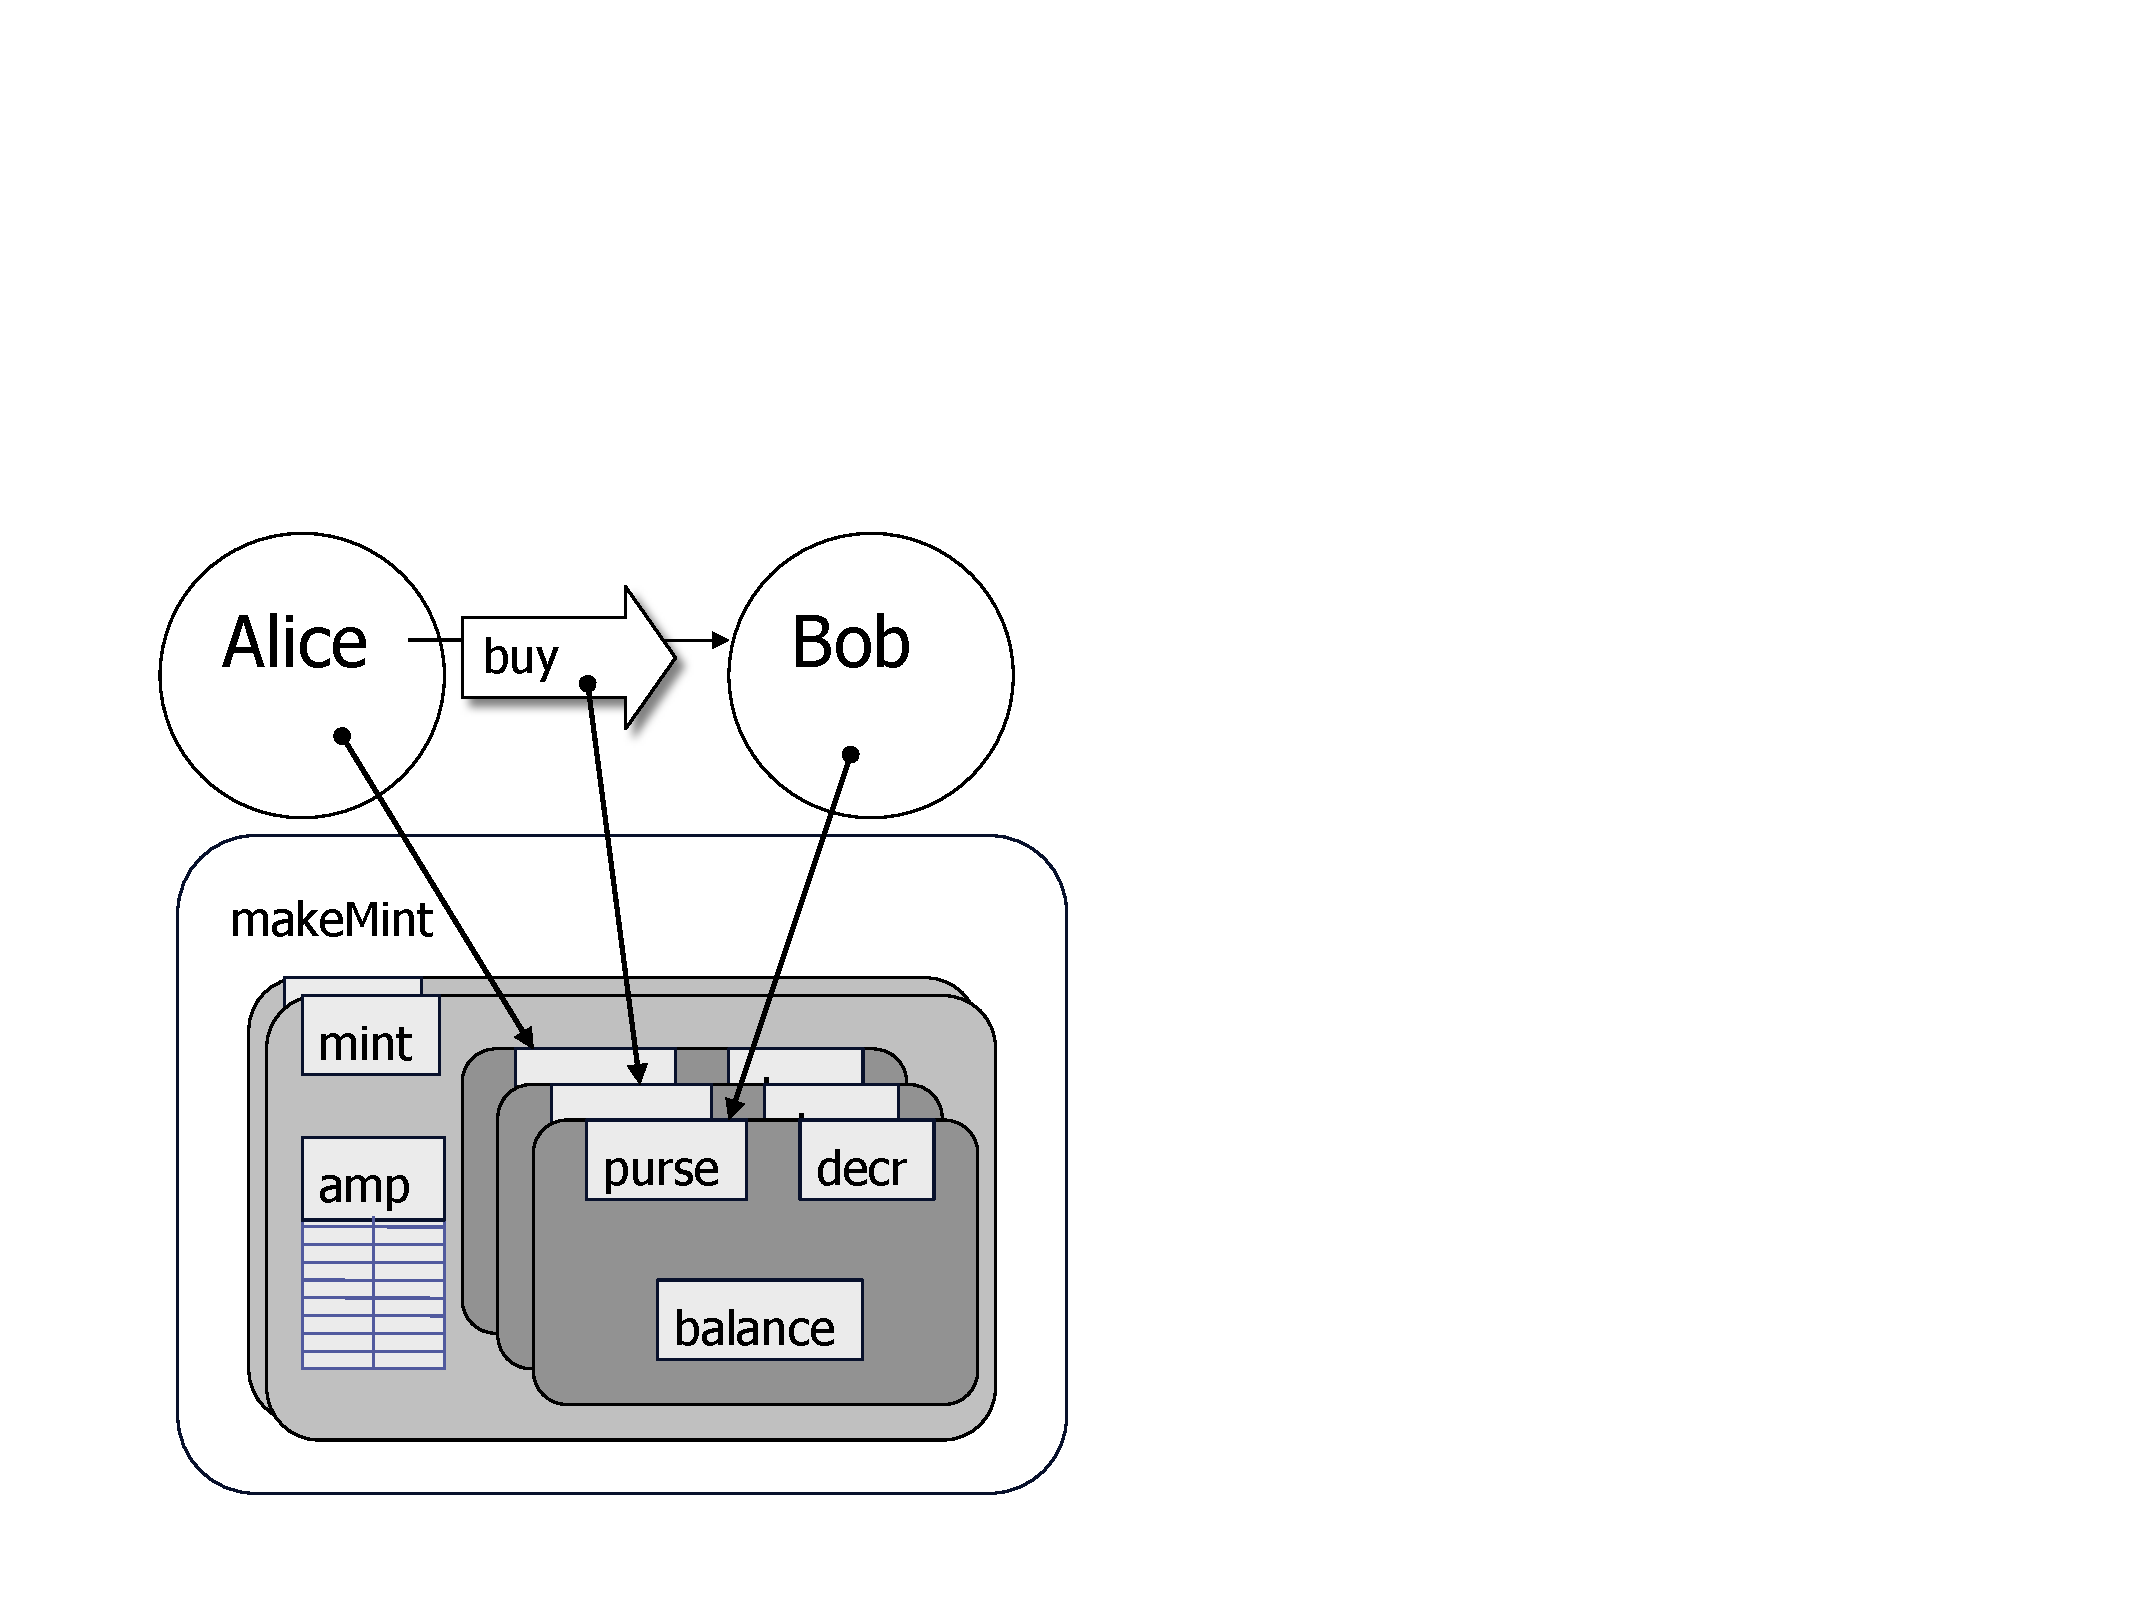
\includegraphics[scale=0.3]{bw-mint.pdf}
\end{minipage}
\caption{The Mint Maker}
\label{makeMint}
\end{figure}

For each currency the bank wishes to manage, the bank calls {\tt makeMint()} once to get a {\tt mint} function for making purses holding units of that currency. When Alice opens an account with, say \$100 in cash, the bank calls {\tt mint(100)} on its \$ mint, to make Alice's main purse. The bank then gives Alice a persistent remote reference to this purse object within the bank.

For Alice to pay Bob, she sets up a \emph{payment purse}, deposits \$10 into it from her main purse, and sends it to Bob in a buy request, together with a description of what she wishes to buy.
\begin{lstlisting}[language=JavaScript,numbers=none]
  var paymentP = myPurse ! makePurse();
  var ackP = paymentP ! deposit(10, myPurse);
  var goodP = ackP.then(_ => bobP ! buy(desc, paymentP));
\end{lstlisting}

On the diagram in Figure~\ref{makeMint}, each {\tt makeMint} call creates a layer with its own ({\tt mint}, {\tt m}) pair representing a distinct currency. Each {\tt mint} call creates a nested layer with its own ({\tt purse}, {\tt decr}, {\tt balance}) triple. On line 16 of the code, each {\tt purse} to {\tt decr} mapping is also entered into the {\tt m} table shared by all purses of the same currency. Alice's main purse is on the bottom purse layer. Bob's is on the top layer. Alice's payment purse, being sent to Bob in the buy message, is in the middle layer.

Bob receives this request at the following {\tt buy} method:

\begin{lstlisting}[language=JavaScript,numbers=none]
  buy: (desc, paymentP) => {
    // do whatever with desc, look up $10 price
    return (myPurse ! deposit(10, paymentP)).then(_ => good);
  }
\end{lstlisting}

Bob's {\tt buy} method handles a message from untrusted clients such as Alice, and thus it does not know what object Alice actually provided as the payment argument. At this point, the purse provided by Alice is \emph{specific}---it is the specific object Alice designated, but to Bob it also is \emph{opaque}. In particular, Bob has no idea if his {\tt paymentP} parameter actually designates a purse, whether it is a purse at this bank, of this currency, and with adequate funds. Even if he knew all these conditions were true at the moment, due to the \emph{shareable} nature of argument passing, Bob wouldn't know the funds would still be there by the time he deposits it. Alice may have retained a reference to it. He delegates all these problems to the bank with the {\tt deposit} request above. 

If the bank's {\tt deposit} method acknowledges a successful deposit, by fulfilling the promise for the result of the deposit, then Bob knows he has obtained \emph{exclusive} access to a \emph{fungible} and \emph{measurable} quantity of a given currency at a given bank. In this case, the success callback of the {\tt .then} above gets called, returning the {\tt good}, fulfilling Alice's pending {\tt goodP} promise.

The interesting work starts on line 11, where {\tt deposit} looks up the alleged payment purse in the {\tt m} table. If this is anything other than a purse of the same currency at the same bank, this lookup will instead return undefined, causing the following function call to throw an error, rejecting Bob's promise for the result of the deposit, rejecting Alice's {\tt goodP}. If this lookup succeeds, it finds the {\tt decr} function for decrementing that purse's {\tt balance}, which it calls with the amount to withdraw. If the payment has insufficient funds, {\tt balance - amount} would be negative and {\tt Nat} would throw.

We have now arrived at the commit point. All the tests that might cause failure have already passed, and no side effects have yet happened. Now we perform all side effects, all of which will happen since no locally observable failure possibilities remain. The assignment decrements the payment purse's {\tt balance} by {\tt amount}, and {\tt decr} returns. Line 12 increments the balance of the purse being deposited into.

The success callback in the {\tt deposit} method implicitly returns undefined, fulfilling Bob's promise for the result of the {\tt deposit} request, triggering Bob to release the good to Alice in exchange.



\section{The Escrow Exchange Contract}
\label{exchange}

\begin{figure}[htbp]
\begin{center}
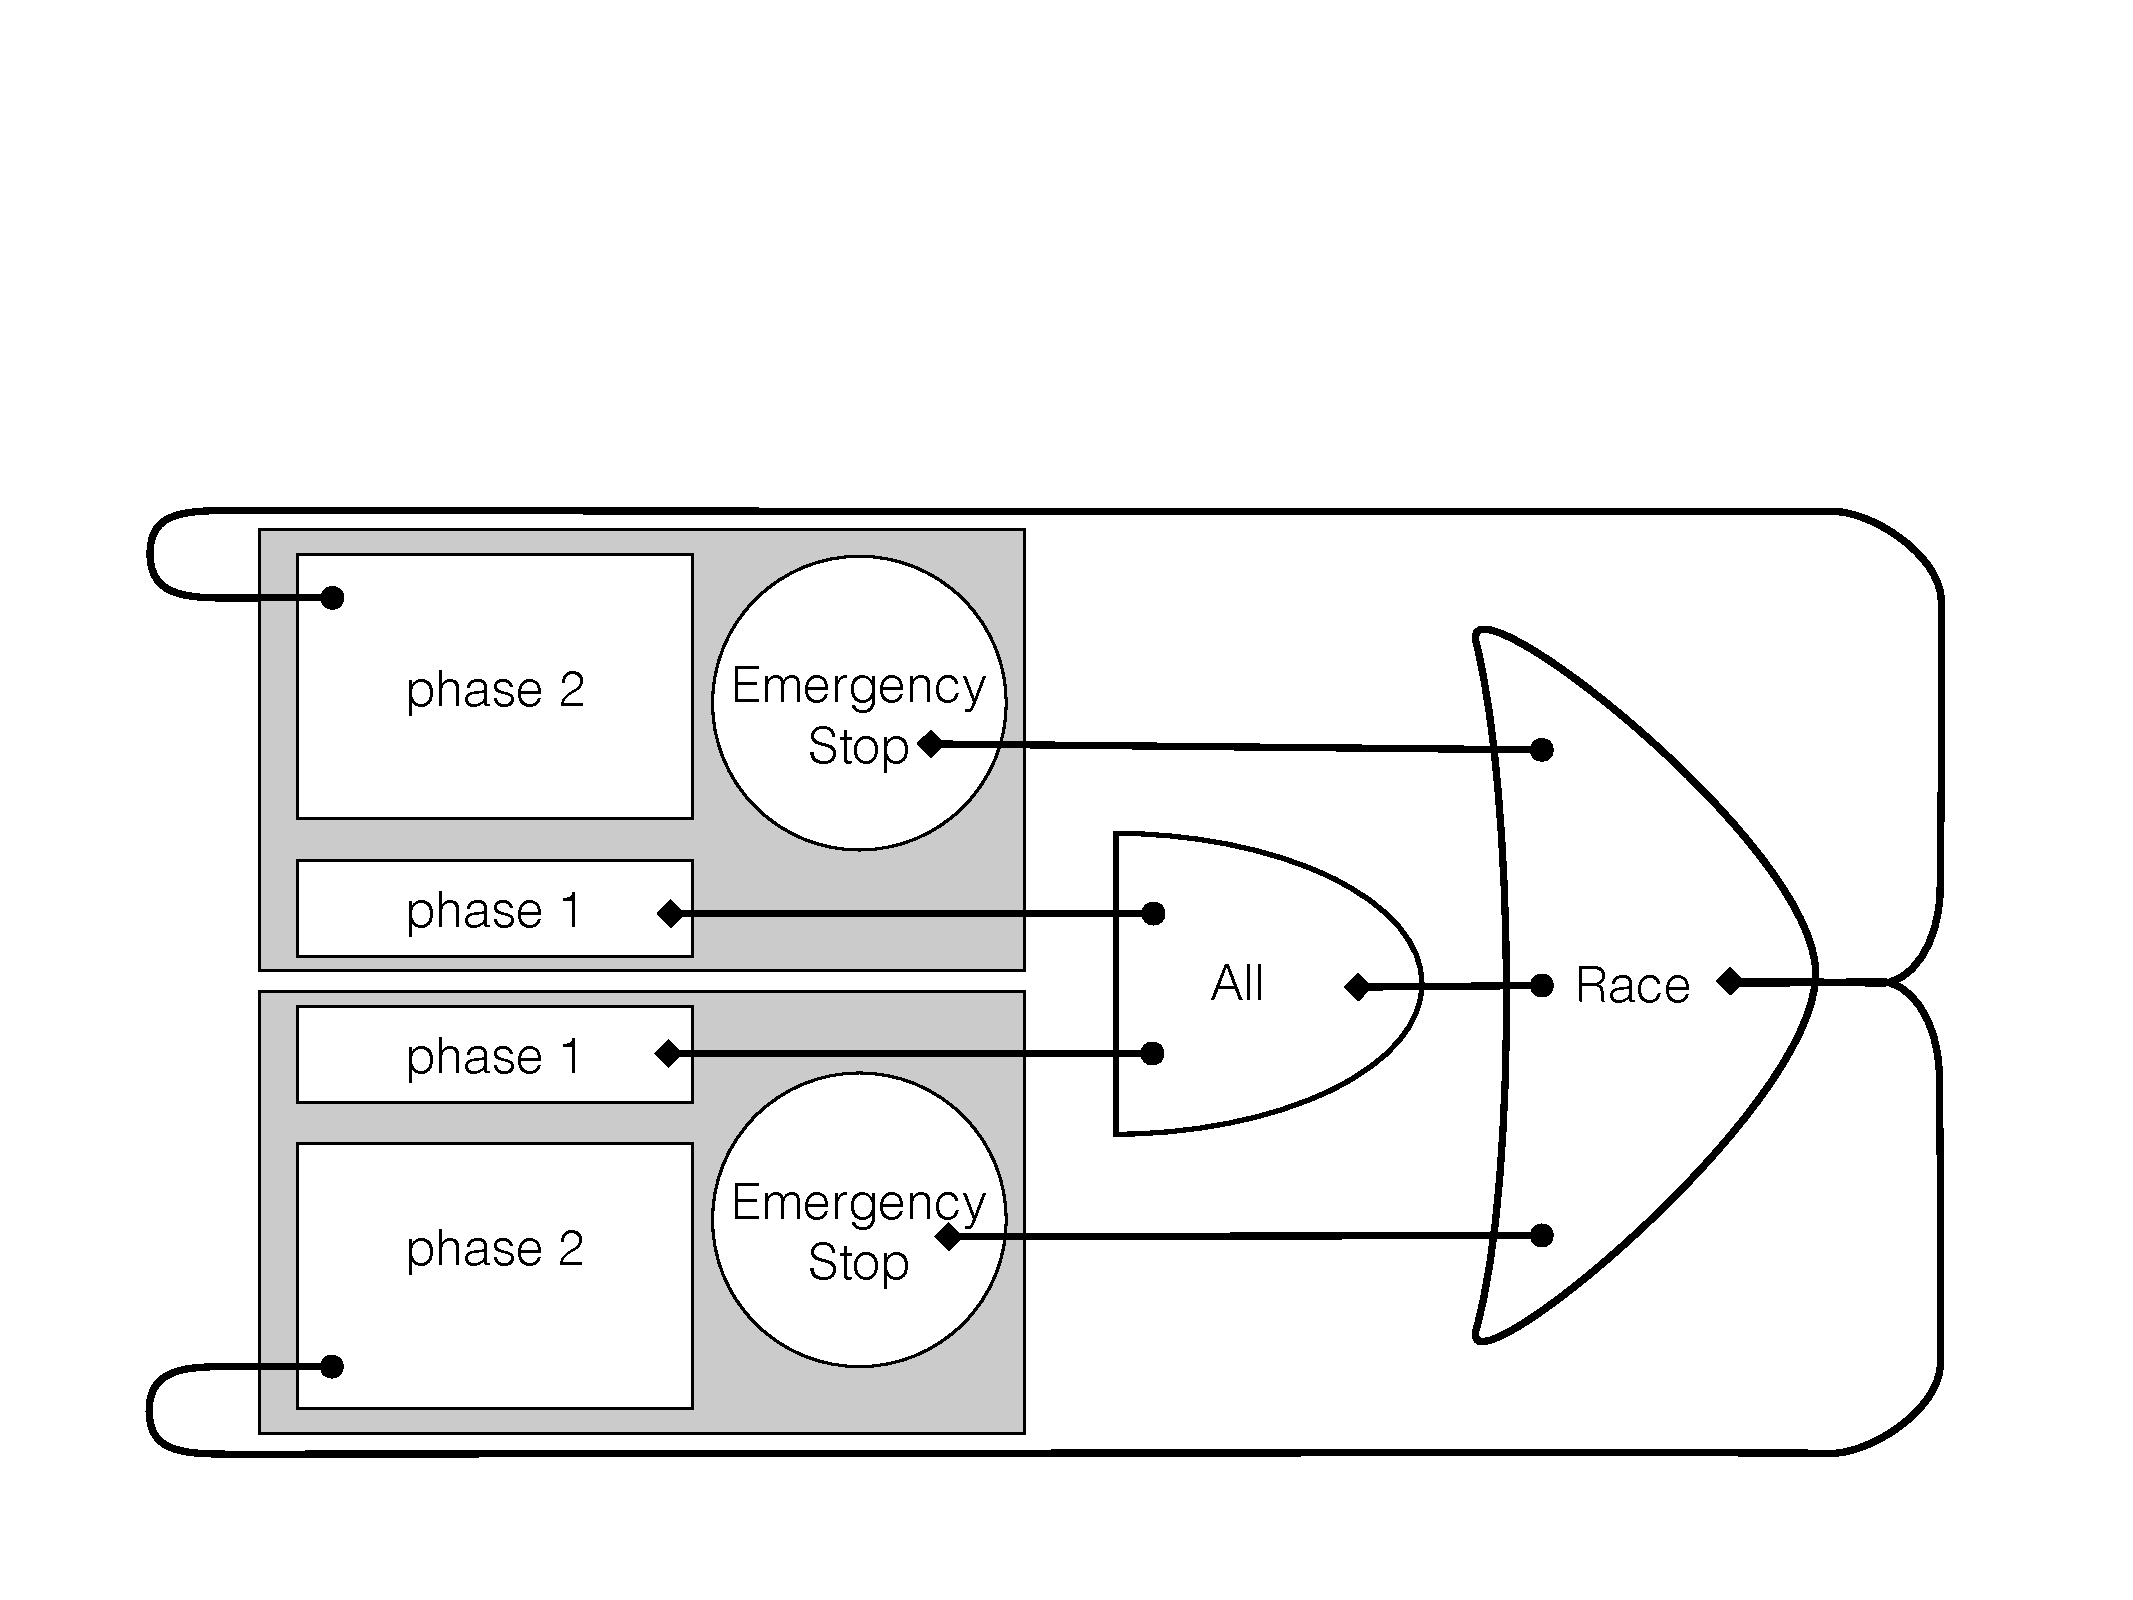
\includegraphics[scale=0.3]{cyclic-circuit.pdf}
\end{center}
\begin{lstlisting}[language=javascript]
var transfer = (decisionP, srcPurseP, dstPurseP, amount) => {
  var makeEscrowPurseP = Q.join(srcPurseP ! makePurse, 
                                          dstPurseP ! makePurse);
  var escrowPurseP = makeEscrowPurseP ! ();

  Q(decisionP).then(                                    // setup phase 2
    _        => { dstPurseP ! deposit(amount, escrowPurseP); },
    reason => { srcPurseP ! deposit(amount, escrowPurseP); });
    
  return escrowPurseP ! deposit(amount, srcPurseP);  // phase 1
};

var failOnly = cancellationP => Q(cancellationP).then(
  cancellation => { throw cancellation; });

var escrowExchange = (a, b) => { // a from Alice, b from Bob
  var decide;
  var decisionP = Q.promise(resolve => { decide = resolve; });

  decide(Q.race([Q.all([
      transfer(decisionP, a.moneySrcP, b.moneyDstP, b.moneyNeeded),
      transfer(decisionP, b.stockSrcP, a.stockDstP, a.stockNeeded)
    ]), 
    failOnly(a.cancellationP), 
    failOnly(b.cancellationP)]));
  return decisionP;
};
\end{lstlisting}
\caption{The Escrow Exchange Contract}
\label{escrowExchange}
\end{figure}

In the mint maker scenario, it is unfortunate that Alice must risk her \$10 on the possibility of Bob's non-delivery. We now introduce an escrow exchange contract that implements an \emph{all or nothing} trade. We explain the escrow exchange contract in terms of a scenario among five players, Alice, Bob, a money issuer running the code of Figure~\ref{makeMint}, a stock issuer also running the code of Figure~\ref{makeMint} but with the units representing shares of some particular stock, and an escrow exchange agent running the code of Figure~\ref{escrowExchange}. The diagram at the top of Figure~\ref{makeContractHost} shows the initial relationships, with the escrow exchange agent in the role of contract host.

Alice and Bob again do not trust each other. They wish to trade \$10 of Alice's money for 7 shares of Bob's stock, but in this case, neither is willing to risk their assets on the possibility of the other's non-delivery. They both trust the same money issuer with their money, the same stock issuer with their stock, and the same escrow exchange agent with the rights to be traded. The money issuer, the stock issuer, and the escrow exchange agent each have no prior knowledge or trust in the others. Additionally, none of these trust Alice or Bob. The rest of the scenario as presented below examines only the consequences of Alice or Bob's misbehavior and assumes the other three run the code shown honestly. A full analysis of vulnerabilities should consider all combinations.

Since the situation is now symmetric, we explain the progression of events from Alice's perspective. Alice's prior trust in each issuer is represented as before---Alice holds a persistent reference to her main purse at each issuer. Alice's prior trust in the escrow exchange agent is represented as the ability to provide the first ``{\tt a}'' argument in the call to {\tt escrowExchange} (Figure~\ref{escrowExchange}, line 12) for which Bob is able to provide the second ``{\tt b}'' argument. Alice might create this argument as follows:

\begin{lstlisting}[language=JavaScript,numbers=none]
  var cancel;
  var a = Q.passByCopy({
    moneySrcP: myMoneyPurse ! makePurse(),
    stockDstP: myStockPurse ! makePurse(),
    stockNeeded: 7,
    cancellationP: Q.promise(r => { cancel = r; });
  });
  a.moneySrcP ! deposit(10, myMoneyPurse);
\end{lstlisting}

By a protocol whose details appear below, Alice sends this ``{\tt a}'' object to the escrow exchange agent, for it to use as the first argument in a call to {\tt escrowExchange}, which initiates this specific contract between Alice and Bob. The {\tt escrowExchange} function returns a promise for the outcome of the contract, which the escrow exchange agent returns to Alice. 

If this outcome promise becomes fulfilled, the exchange succeeded,  she should expect her {\tt a.moneySrcP} to be drained, and 7 shares of stock to be deposited into her {\tt a.stockDstP} promptly.\footnote{
%
By "promptly" we mean, once the relevant machines are up, processes running, and reachable to each other over the network.
%
} If this promise becomes rejected, the exchange failed, and she should expect her \$10 to reappear in her {\tt a.moneySrcP} promptly. In the meantime, if she gets impatient and would rather not continue waiting, she can call her {\tt cancel} function with her alleged reason for walking away. Once she does so, the exchange will then either succeed or fail promptly.

On lines 13 and 14 of Figure~\ref{escrowExchange} the {\tt escrowExchange} contract makes a {\tt decisionP} promise whose fulfillment or rejection represents its decision about whether the exchange must succeed or fail. It makes this decision by calling {\tt decide} with the outcome of a race between a {\tt Q.all} and two calls to {\tt failOnly}. Until a player cancels the exchange, the {\tt Q.race} can only be won by the {\tt Q.all}, which is where the exchange is proceeding.

The arguments to {\tt Q.all} are the results of two calls to {\tt transfer}. The first call to {\tt transfer} sets up activity whose purpose is to transfer money from Alice to Bob. The second call's purpose is to transfer stock from Bob to Alice. Each call to transfer returns a promise whose fulfillment or rejection indicates whether it has become confident that this one-way transfer of erights would succeed. If both transfers become confident (before any cancellations win the race), then the overall decision is to proceed. If either transfer indicates failure, by rejecting the promise it has returned, then, via {\tt Q.all}, {\tt decisionP} becomes rejected.\footnote{
%
This pattern implements two phase commit enhanced with the possibility of cancellation, where the call to {\tt escrowExchange} creates a transaction coordinator, and each of its calls to {\tt transfer} creates a participant.}

We do not feed the cancellation promises directly into the race, as Alice could then fulfill the cancellation promise, causing the race to signal a decision to proceed with the exchange, even though Alice's money has not been escrowed, potentially giving Bob's stock to Alice for free. Instead, once the cancellation promise has been either fulfilled or rejected, the promise returned by {\tt failOnly} will only become rejected. Only the {\tt Q.all} can win the race with a success.

Since the two calls to {\tt transfer} are symmetric, we examine only the first. The first phase of the transfer, on line 8 of Figure~\ref{escrowExchange}, attempts to deposit Alice's money into an escrow purse mentioned only within this transfer. If this deposit succeeds, Alice's money has been escrowed, so the money portion of the exchange is now assured. If this deposit fails, then the exchange as a whole should be cancelled. So {\tt transfer} simply returns the promise for the outcome of this first deposit.

The {\tt transfer} function sets up the second phase on lines 5, 6, and 7. If the overall decision is that the exchange should succeed,  the success callback deposits Alice's escrowed money into Bob's account. Otherwise it refunds Alice's money.

Only one mystery remains. How does the escrow agent obtain a fresh escrow purse at this money issuer, in order to be confident that it has obtained exclusive access to the money at stake? Since the escrow exchange agent has no prior knowledge or trust in the money issuer, it cannot become confident that the issuer is honest or even that the money it issues means anything. The question is meaningless. Instead, it only needs to obtain a fresh escrow purse whose veracity is \emph{mutually acceptable} to Alice and Bob.

If the escrow contract simply asks Alice's purse for a new empty purse ({\tt srcPurseP~!~makePurse()}), Alice could return a dishonest purse that acknowledges deposit without transferring anything. Alice would then obtain Bob's stock for free. If it simply asks Bob's purse, then Bob could steal Alice's money during phase 1. Instead, it checks if their {\tt makePurse} methods are the very same function object---have the same object identity---by using {\tt Q.join} on promises for these two methods. This is why, on lines 3 and 7 of Figure~\ref{makeMint}, all purses of the same currency at the same bank share the same function as their {\tt makePurse} method. If the {\tt Q.join} of these two methods fails, then either Alice was dishonest, Bob was dishonest, or they simply didn't have prior agreement on the same currency at the same money issuer.

\section{The Contract Host}
\label{contracthost}

\begin{figure}[htbp]
\begin{minipage}[t]{0.52\linewidth}
\begin{lstlisting}[language=javascript]
var makeContractHost = () => {
  var m = WeakMap();

  return def({
    setup: contractSrc => {
      contractSrc = ''+contractSrc;
      var tokens = [];
      var argPs = [];
      var resolve;
      var resultP = Q.promise(r => { resolve = r; });
      var contract = confine(contractSrc, {Q: Q});

      var addParam = (i, token) => {
        tokens[i] = token;
        var resolveArg;
        argPs[i] = Q.promise(r => { resolveArg = r; });
        m.set(token, (allegedSrc, allegedI, arg) => {
          if (contractSrc !== allegedSrc) {
            throw new Error('unexpected contract: '+contractSrc);
          }
          if (i !== allegedI) {
            throw new Error('unexpected side: '+i);
          }
          m.delete(token);
          resolveArg(arg);
          return resultP;
        });
      };
      for (var i = 0; i < contract.length; i++) {
        addParam(i, def({}));
      }
      resolve(Q.all(argPs).then(
        args => contract.apply(undefined, args)));
      return tokens;
    },
    play: (tokenP, allegedSrc, allegedI, arg) => Q(tokenP).then(
      token => m.get(token)(allegedSrc, allegedI, arg))
  });
};
\end{lstlisting}
\end{minipage}
\begin{minipage}[t]{0.48\linewidth}
\vspace{0pt}
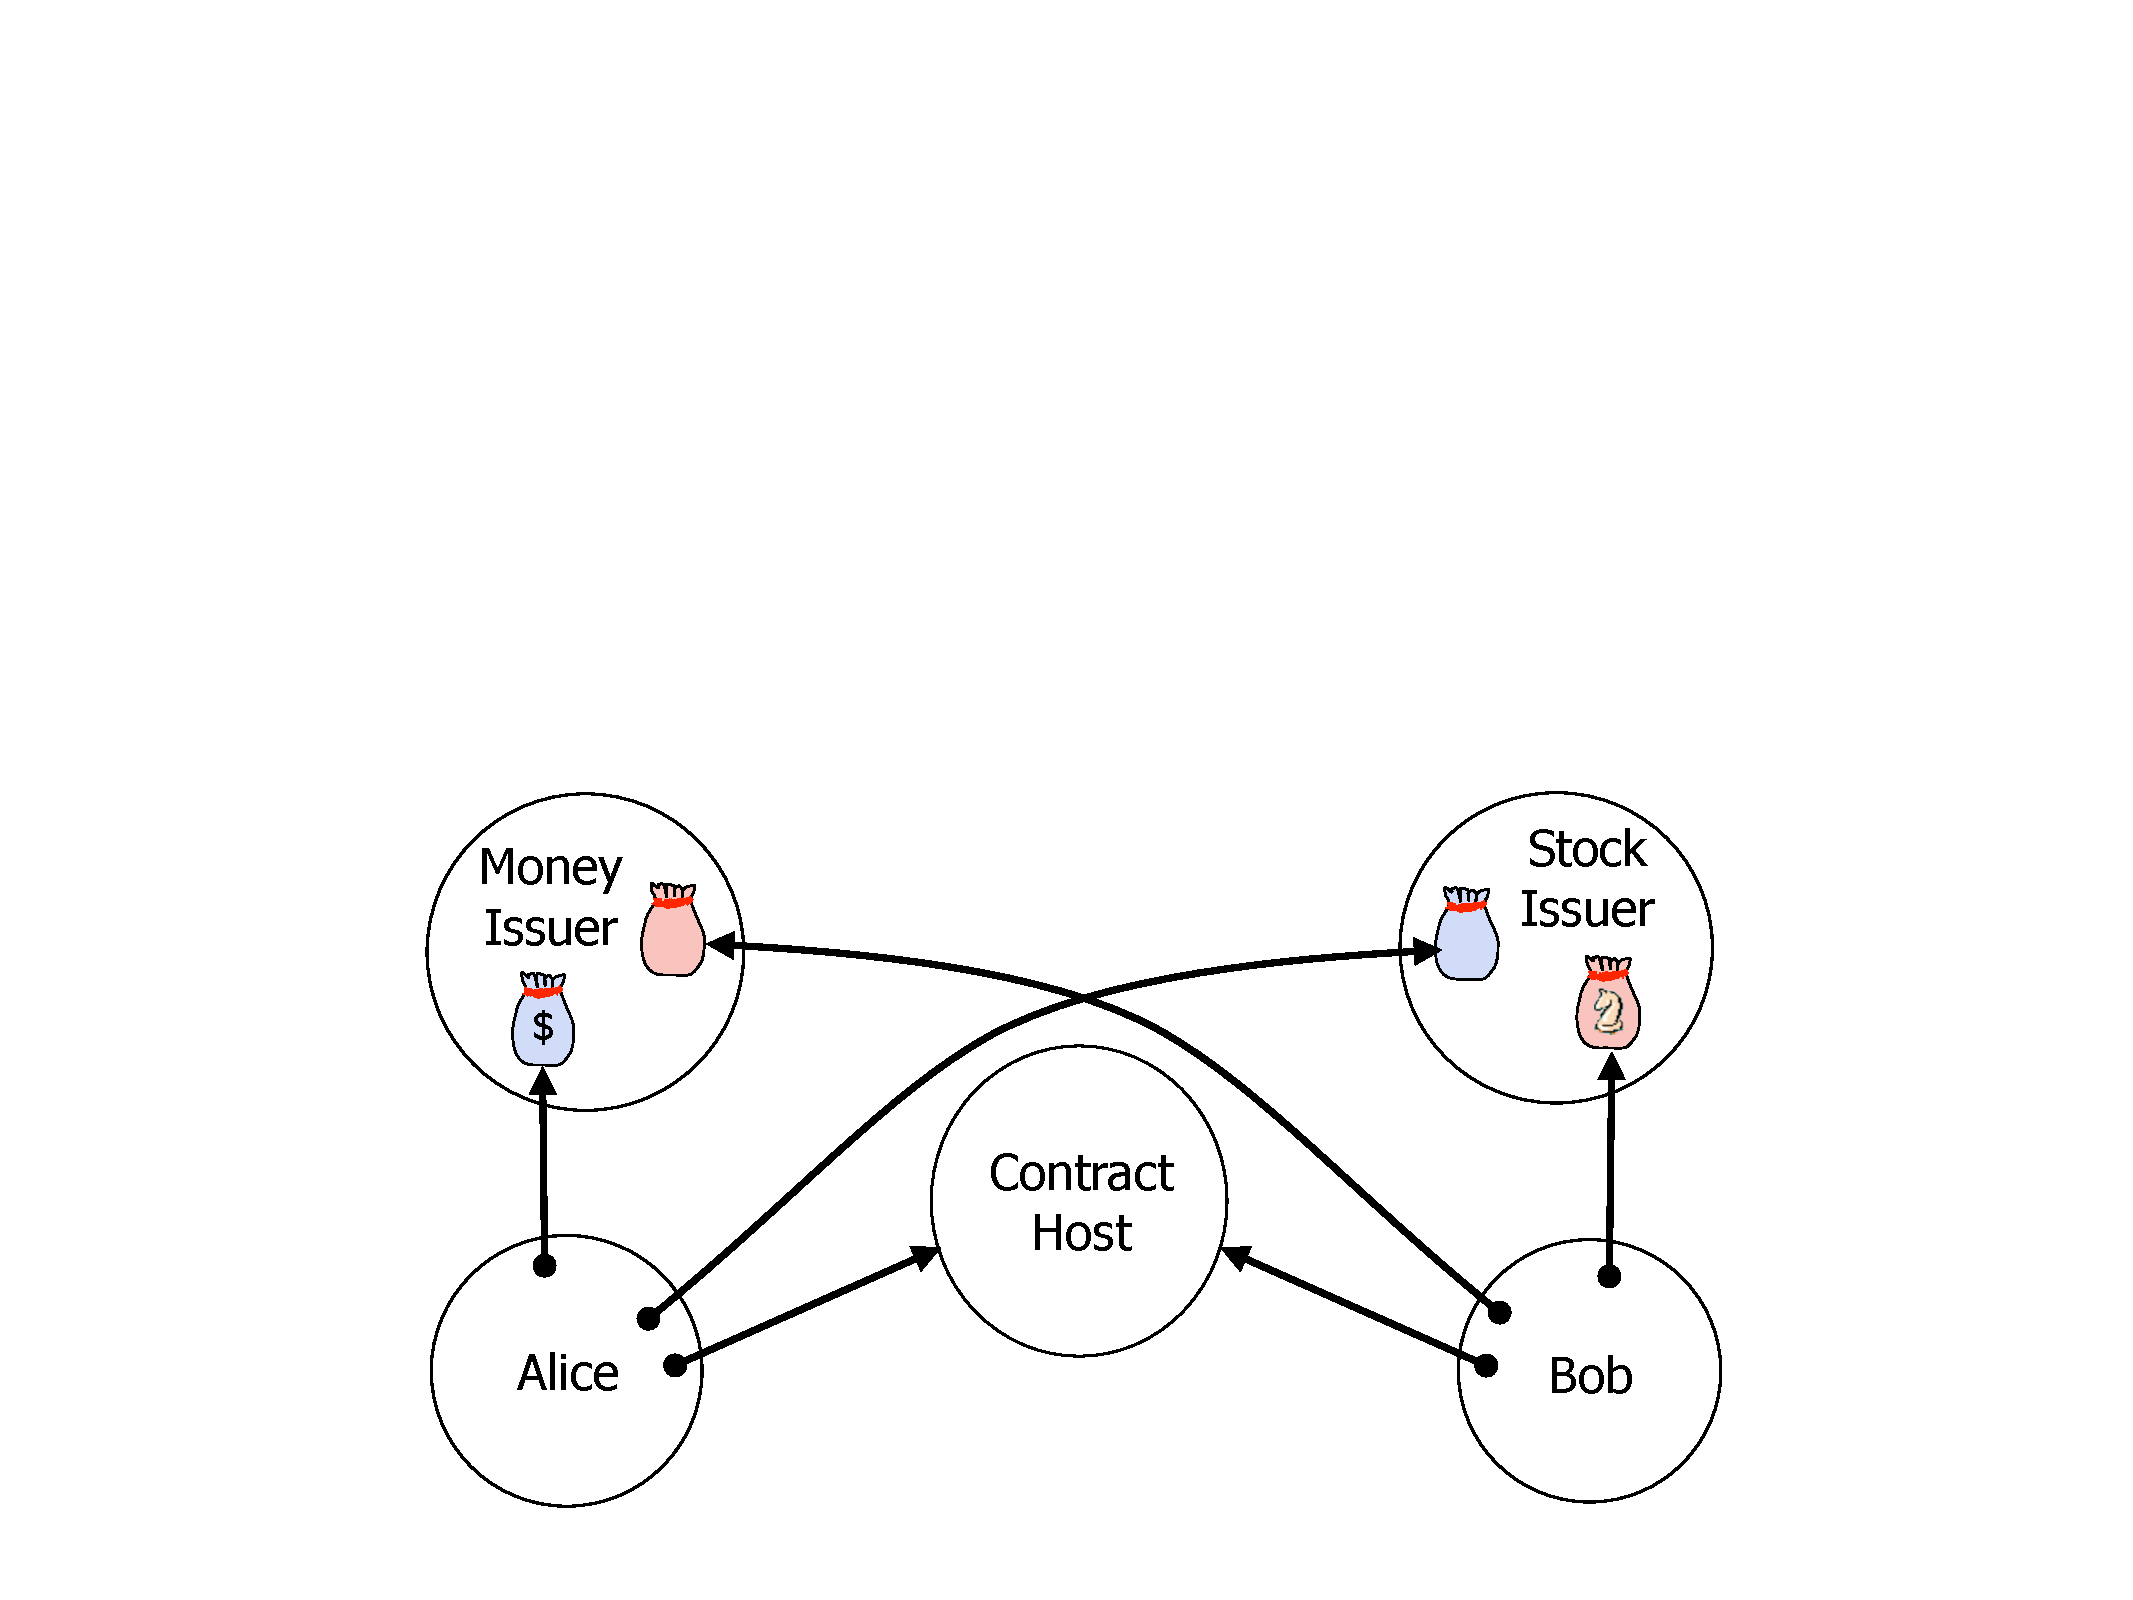
\includegraphics[scale=0.26]{5players.pdf}
\end{minipage}
\caption{The Contract Host}
\label{makeContractHost}
\end{figure}

Once Alice and Bob agree on a contract, how do they arrange for it to be run in a mutually trusted manner?

To engage in the escrow exchange contract, Alice and Bob had to agree on the issuers, which is unsurprising since they need to agree on the nature of rights exchanged by the contract. And they had to agree on an escrow exchange agent to honestly run the escrow exchange contract specifically. For a contract as general as this, perhaps that is not a problem. But if Alice and Bob negotiate a custom contract specialized to their needs, they should not expect to find a mutually trusted third party specializing in running this particular contract. Rather, it should be adequate for them to agree on:

\begin{itemize}
\renewcommand{\labelitemi}{$\bullet$}
\item The issuers of each of the rights at stake.
\item The source code of the contract.
\item Who is to play which side of the contract.
\item A third party they mutually trust to run their agreed code, \emph{whatever it is}, honestly.
\end{itemize}

Figure~\ref{makeContractHost} shows the code for a generic contract host. It is able to host any contract formulated, as our escrow exchange contract is, as a function, taking one argument from each player and returning the outcome of the contract as a whole. Setting up a contract involves a necessary asymmetry among the players. One of the players, say Bob, must initiate a new live contract instance by sending the contract's code to the contract host. At this point, only Bob knows both this contract instance and that he'd like to invite Alice to participate in \emph{this} instance. If Bob simply sent to Alice references to those objects on the contract host that enable Alice to play, Alice would not know what she's received, since she received it from Bob whom she does not trust. She does trust the contract host, and these objects are on the contract host, but so are the objects corresponding to other contracts this host is initiating or running. Only Bob can connect Alice to this contract instance, but Alice's confidence that she's playing the contract she thinks she is must be rooted in her prior trust in the contract host.

Our contract host is an object with two methods, {\tt setup} and {\tt play}. Bob sets up the contract instance by calling {\tt setup} with the source code for the contract function in question, e.g., {\tt escrowExchange}. At line 32, {\tt setup} returns an array of unique unforgeable tokens, one for each contract parameter. Bob's invitation to Alice includes this token, the source for the contract he wishes Alice to play, the argument index indicating what side of the contract Alice is to play, and the contract host in question.

If Alice decides she'd like to play this contract, she formulates her argument object as above, and sends it in a {\tt play} request to the contract host along with the token, the alleged contract source code, and the alleged side she is to play. If all of this checks out and this token has not previously been redeemed, then this token gets used up, Alice's argument is held until the arguments for the other players arrive, and Alice receives a promise for the outcome of the contract. Once all arguments arrive, the contract function is called and its result is used to resolve the previously returned promise.

By redeeming the token, Alice obtains the exclusive right to play a specific contract whose logic she knows, and whose play she expects to cause external effects. This eright is exclusive, specific, measurable, and exercisable. 

\section*{Conclusions}
\label{conclusions}

In human society, rights are a scalable means for organizing the complex cooperative interactions of decentralized agents with diverse interests. This perspective is helping us shape JavaScript into a distributed resilient secure programming language. We show how this platform would enable the expression of new kinds of rights and smart contracts \emph{simply}, supporting new forms of cooperation among computational agents.



\paragraph{Acknowledgements}

Many people contributed to the progress reported here, including the e-lang community for refining ocap-based smart contracting, the Google Caja group where SES started, TC39 for making ES5 and successors friendly to ocaps, Tyler Close for the first Ken and Q, Terence Kelly for the new Ken, and Kris Kowal for the new Q. 

Tom Van Cutsem is a post-doctoral fellow of the Research Foundation, Flanders. Thanks to Terry Stanley, Kevin Reid, and Terence Kelly for suggestions improving this paper.

\bibliographystyle{splncs}
% \bibliographystyle{alpha}
\bibliography{common}

\end{document}































